\documentclass[../defence.tex]{subfiles}
\newcommand*{\NewNumbers}{%
   \pgfmathsetmacro{\A}{random(0,580)}
   \pgfmathsetmacro{\B}{random(0,26)}}
\begin{document}
  \begin{frame}{Atomic layer deposition (ALD)}
    \begin{columns}[onlytextwidth, T]
      \column{\dimexpr\linewidth / 21 * 10}
        \only<1->{\scalebox{0.6}{
          \tikzsetnextfilename{ald-1}
          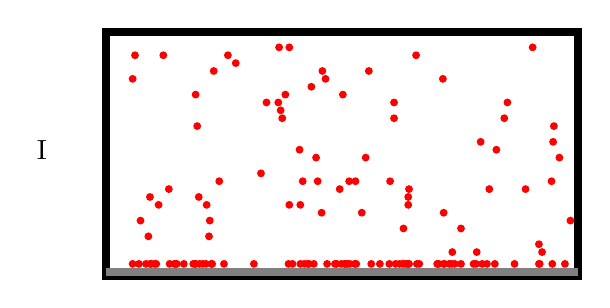
\begin{tikzpicture}
            \node[anchor=west] at (-4,0) {I};
            \draw[color=black, line width=1mm] (-3,-1.6) rectangle (3,1.5);
            \foreach \x in {1,...,70}{
              \NewNumbers
              \fill[red] (\A / 100 - 290 / 100,\B / 10 - 13 / 10) circle (0.5mm);
            }
            \foreach \x in {1,...,70}{
              \NewNumbers
              \fill[red] (\A / 100 - 290 / 100,-1.45) circle(0.5mm);
            }
            \fill[gray] (-3,-1.6) rectangle (3,-1.5);
          \end{tikzpicture}}}
        \only<3->{\scalebox{0.6}{
          \tikzsetnextfilename{ald-3}
          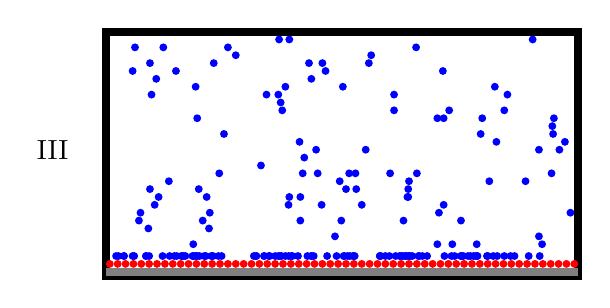
\begin{tikzpicture}
            \node[anchor=west] at (-4,0) {III};
            \draw[color=black, line width=1mm] (-3,-1.6) rectangle (3,1.5);
            \fill[gray] (-3,-1.6) rectangle (3,-1.5);
            \foreach \x in {-2.95,-2.85,...,2.95}{
              \fill[red] (\x,-1.45) circle(0.5mm);
            }
            \begin{scope}[yshift=0.1cm]
              \foreach \x in {1,...,100}{
                \NewNumbers
                \fill[blue] (\A / 100 - 290 / 100,\B / 10 - 13 / 10) circle(0.5mm);
              }
            \end{scope}
            \foreach \x in {1,...,100}{
              \NewNumbers
              \fill[blue] (\A / 100 - 290 / 100,-1.35) circle(0.5mm);
            }
          \end{tikzpicture}}}
        \only<5->{\scalebox{0.6}{
          \tikzsetnextfilename{ald-5}
          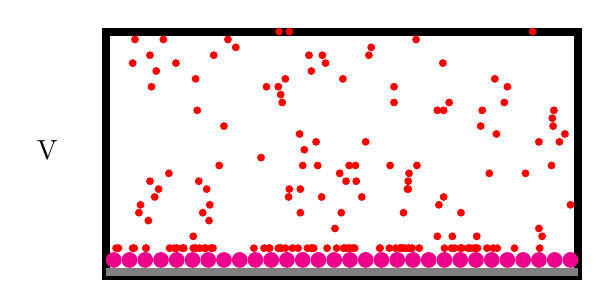
\begin{tikzpicture}
            \node[anchor=west] at (-4,0) {V};
            \draw[color=black, line width=1mm] (-3,-1.6) rectangle (3,1.5);
            \fill[gray] (-3,-1.6) rectangle (3,-1.5);
            \foreach \x in {-2.9,-2.7,...,2.9}{
              \fill[magenta] (\x,-1.4) circle(1mm);
            }
            %\foreach \x in {-2.95,-2.85,...,2.95}{
            %  \fill[blue] (\x,-1.35) circle(0.5mm);
            %}
            \begin{scope}[yshift=0.2cm]
              \foreach \x in {1,...,100}{
                \NewNumbers
                \fill[red] (\A / 100 - 290 / 100,\B / 10 - 13 / 10) circle(0.5mm);
              }
            \end{scope}
            \foreach \x in {1,...,70}{
              \NewNumbers
              \fill[red] (\A / 100 - 290 / 100,-1.25) circle(0.5mm);
            }
          \end{tikzpicture}}}

      \column{\dimexpr\linewidth / 21}
      \column{\dimexpr\linewidth / 21 * 10}
        \only<2->{\scalebox{0.6}{
          \tikzsetnextfilename{ald-2}
          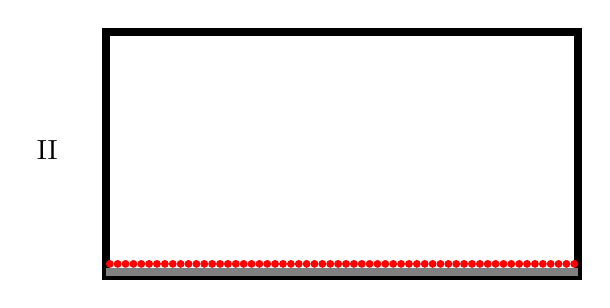
\begin{tikzpicture}
            \node[anchor=west] at (-4,0) {II};
            \draw[color=black, line width=1mm] (-3,-1.6) rectangle (3,1.5);
            \fill[gray] (-3,-1.6) rectangle (3,-1.5);
            \foreach \x in {-2.95,-2.85,...,2.95}{
              \fill[red] (\x,-1.45) circle(0.5mm);
              }
          \end{tikzpicture}}
          }
        \only<4->{\scalebox{0.6}{
          \tikzsetnextfilename{ald-4}
          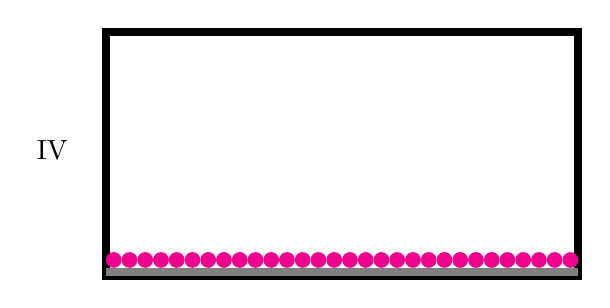
\begin{tikzpicture}
            \node[anchor=west] at (-4,0) {IV};
            \draw[color=black, line width=1mm] (-3,-1.6) rectangle (3,1.5);
            \fill[gray] (-3,-1.6) rectangle (3,-1.5);
            \foreach \x in {-2.9,-2.7,...,2.9}{
              \fill[magenta] (\x,-1.4) circle(1mm);
            }
          %  \foreach \x in {-2.95,-2.85,...,2.95}{
          %    \fill[blue] (\x,-1.35) circle(0.5mm);
          %}
        \end{tikzpicture}}}
        \only<6->{\scalebox{0.6}{
          \tikzsetnextfilename{ald-6}
          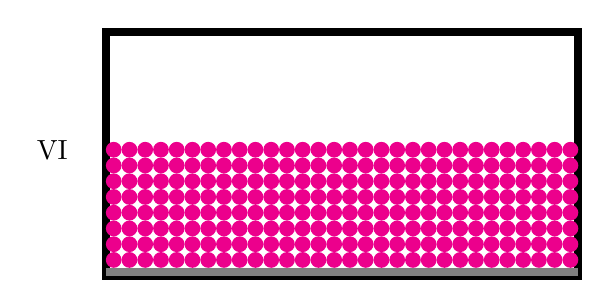
\begin{tikzpicture}
            \node[anchor=west] at (-4,0) {VI};
            \draw[color=black, line width=1mm] (-3,-1.6) rectangle (3,1.5);
            \fill[gray] (-3,-1.6) rectangle (3,-1.5);
            \foreach \y in {-1.4,-1.2,...,0}{
              \foreach \x in {-2.9,-2.7,...,2.9}{
                \fill[magenta] (\x,\y) circle(1mm);
              }
            }
          \end{tikzpicture}}
          }
    \end{columns}
  \end{frame}
\end{document}
